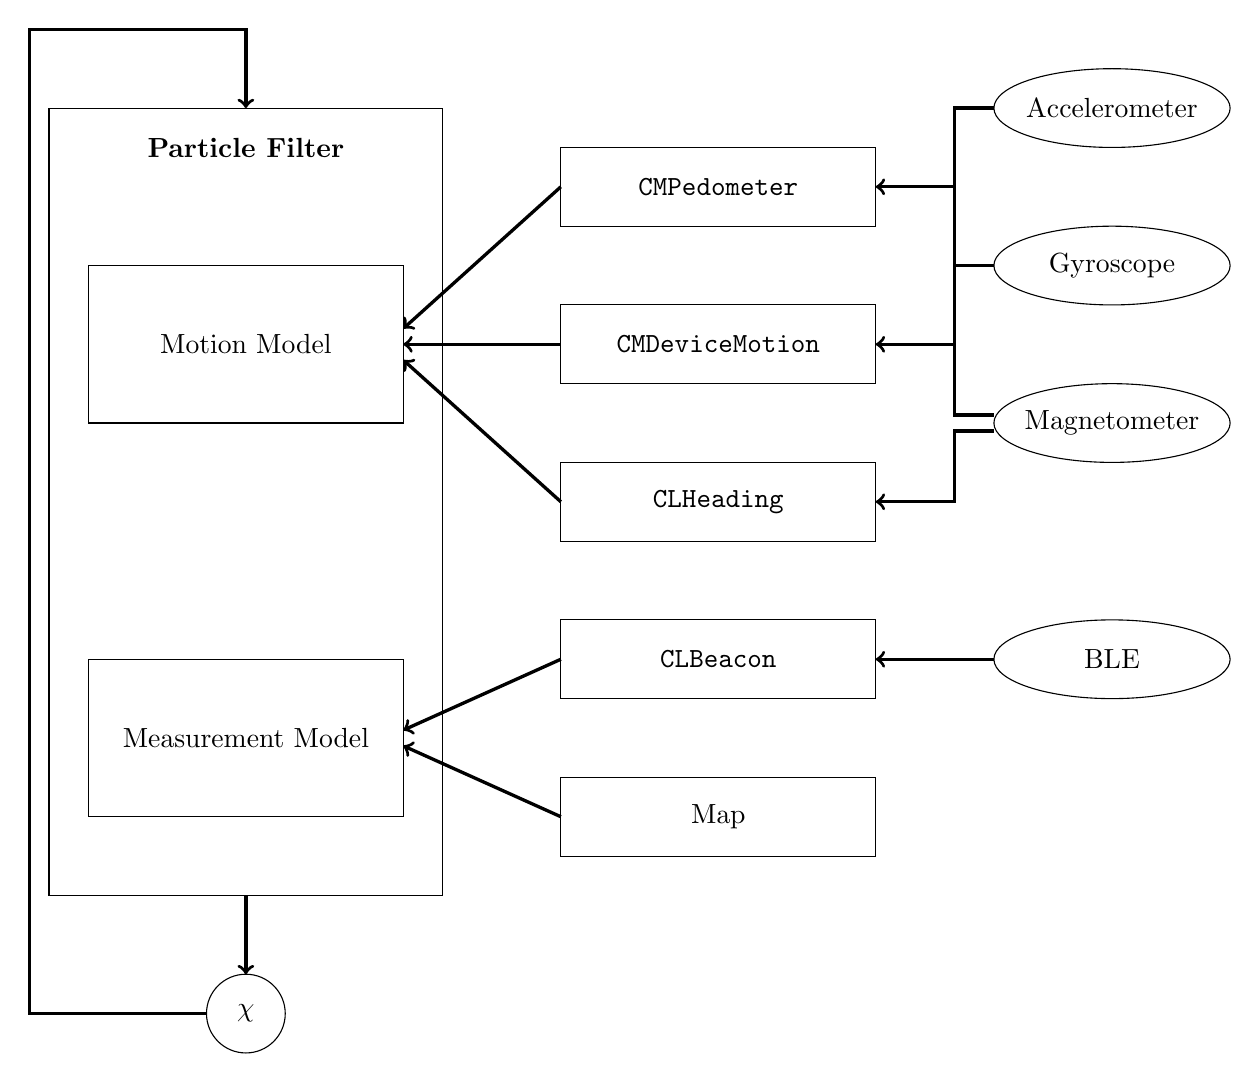
\begin{tikzpicture}
 %\draw[style=help lines] (0,0) grid (15,10);

 % sensors
 \node (A) at (13,9) {Accelerometer};
 \node (G) at (13,7) {Gyroscope};
 \node (M) at (13,5) {Magnetometer};
 \node (B) at (13,2) {\acs{BLE}};

 \draw (A) ellipse (1.5 and 0.5);
 \draw (G) ellipse (1.5 and 0.5);
 \draw (M) ellipse (1.5 and 0.5);
 \draw (B) ellipse (1.5 and 0.5);

 % Frameworks
 \node (CMP) at (8,8) {\texttt{CMPedometer}};
 \node (CMDM) at (8,6) {\texttt{CMDeviceMotion}};
 \node (CLH) at (8,4) {\texttt{CLHeading}};
 \node (CLB) at (8,2) {\texttt{CLBeacon}};
 \node (MAP) at (8,0) {Map};

 \draw (6,7.5) rectangle (10,8.5);
 \draw (6,5.5) rectangle (10,6.5);
 \draw (6,3.5) rectangle (10,4.5);
 \draw (6,1.5) rectangle (10,2.5);
 \draw (6,-0.5) rectangle (10,0.5);


 \draw[very thick] (11.5,9) -- ++(-0.5,0) -- ++(0,-2) -- ++(0.5,0) -- ++(-0.5,0) -- ++(0,-1.9) -- ++(0.5,0);
 \draw[->, very thick] (11,8) to (10,8);
 \draw[->, very thick] (11,6) to (10,6);


 \draw[->, very thick] (11.5,4.9) -- ++(-0.5,0) -- ++(0,-0.9) -- ++(-1,0);
 \draw[->, very thick] (11.5,2) to (10,2);

 % Particle Filter
 \draw (-0.5,-1) rectangle (4.5,9);
 \node (MM) at (2,8.5) {\textbf{Particle Filter}};

 % Motion Model
 \draw (0,5) rectangle (4,7);
 \node (MM) at (2,6) {Motion Model};

 \draw[->, very thick] (6,8) to (4,6.2);
 \draw[->, very thick] (6,6) to (4,6);
 \draw[->, very thick] (6,4) to (4,5.8);

 % Measurement Model
 \draw (0,0) rectangle (4,2);
 \node (MM) at (2,1) {Measurement Model};

 \draw[->, very thick] (6,2) to (4,1.1);
 \draw[->, very thick] (6,0) to (4,0.9);

 % Location
 \node (L) at (2,-2.5) {$\chi$};
 \draw (L) ellipse (0.5 and 0.5);
 \draw[->, very thick] (2,-1) -- ++(0,-1);
 \draw[->, very thick] (1.5,-2.5) -- ++(-2.25,0) -- ++(0,12.5) -- ++(2.75,0) -- ++(0,-1);

\end{tikzpicture}
